\documentclass{beamer}

%%%%%%%%%%%%%%%%%%%%%%%%%%%%%%%%%%
% PAKCAGES
%%%%%%%%%%%%%%%%%%%%%%%%%%%%%%%%%%

\usepackage{etoolbox}
\usepackage{xparse}
\usepackage{graphicx}
\usepackage{subcaption}
\usepackage{moresize}
\usepackage{anyfontsize}
\usepackage{bm} %use bold in math
\usepackage{tikz}
\usepackage[utf8]{inputenc}
\usepackage[english]{babel}
\usepackage{xcolor}
\usepackage{cancel} % use xcancel see https://jansoehlke.com/2010/06/strikethrough-in-latex/

\usepackage{calculator}



\makeatletter

\NewDocumentCommand{\setFontSize}{m o m}{%
    \IfNoValueF{#2}{%
        \fontsize{#1}{#2}\selectfont#3%
    }{%
        % see https://texblog.org/2012/08/29/changing-the-font-size-in-latex/
        \MULTIPLY{#1}{1.2}{\setFont@baseline}%
        \fontsize{#1}{\setFont@baseline}\selectfont#3%
    }%
}

\NewDocumentCommand{\todo}{m}{%
    {\color{blue} #1}%
}

\NewDocumentCommand{\code}{m}{%
    \texttt{#1}%
}

\makeatother
\NewDocumentCommand{\CPD}{}{%
    \texttt{CPD}%
}

\NewDocumentCommand{\ALT}{}{%
    \texttt{ALT}%
}

\NewDocumentCommand{\AWA}{}{%
    \texttt{AWA$^*$}%
}

\NewDocumentCommand{\WA}{}{%
    \texttt{WA$^*$}%
}

\NewDocumentCommand{\A}{}{%
    \texttt{A$^*$}%
}

\NewDocumentCommand{\CPDSearch}{}{%
    \texttt{CPD-Search}%
}

\NewDocumentCommand{\anytimeCPDSearch}{}{%
    \texttt{Anytime CPD-Search}%
}


\NewDocumentCommand{\CPDPathName}{}{%
    \texttt{CPD}-Path%
}

\NewDocumentCommand{\CPDPathsName}{}{%
    \texttt{CPD}-Paths%
}

\NewDocumentCommand{\CPDPath}{m m}{%
    \texttt{CPD-Path}[#1, #2]%
}

\NewDocumentCommand{\CPDPathCostOriginal}{m m}{%
    \ifmmode{h_{CPD}[#1]}\else{$h_{CPD}[#1]$}\fi%
}

\NewDocumentCommand{\CPDPathCostNew}{m m}{%
    \ifmmode{h'_{CPD}[#1]}\else{$h'_{CPD}[#1]$}\fi%
}

\NewDocumentCommand{\pathOnGraph}{m m}{%
    path[#1, #2]%
}

\NewDocumentCommand{\pathCostOnGraph}{m m}{%
    cost(path[#1, #2])%
}


%%%%%%%%%%%%%%%%%%%%%%%%%%%%%%%%%%%%%%%
% CONFIGURATIONS
%%%%%%%%%%%%%%%%%%%%%%%%%%%%%%%%%%%%%%%

%beamer theme
\usetheme{Frankfurt}

\setbeamertemplate{itemize item}{$\bm{\diamond}$}

\title{Path Planning with CPD Heuristics}
\author{Massimo Bono$^1$, Alfonso E. Gerevini$^1$, Daniel D. Harabor$^2$ and Peter J.Stuckey$^2$}
\institute{%
    $^1$\setFontSize{7.8}{Dipartimento di Ingegneria dell'Informazione, Università degli Studi di Brescia, Italy}%
    \\%
    $^2$\setFontSize{7.8}{Faculty of Information Technology, Monash University, Melbourne, Australia}%
    \\%
    \{mbono, alfonso.gerevini\}@unibs.it, \{daniel.harabor, peter.stuckey\}@monash.edu%
}
%\date{\today}
\date{August 15, 2019}

\setInputPath{%
    {src/texs}%
    {src/images}%
    {src/tikzs}%
    {src/bibs}%
}

%%%%%%%%%%%%%%%%%%%%%%%%%%%%%%%%%%%%%%%%%%%%
% DOCUMENT
%%%%%%%%%%%%%%%%%%%%%%%%%%%%%%%%%%%%%%%%%%%%

\begin{document}

%https://stackoverflow.com/a/3210406/1887602
\beamertemplatenavigationsymbolsempty

% tempo totale: 13 minuti => 50 secondi per slide! è chiaro che qualche slide va rimossa
% High level
% SLIDE 1: titolo
% SLIDE 2: 
%    - path finding è importante (videogiochi, routing); moderne soluzioni usano auxiliary data per calcolare velocemente;
%    - una variante del problema è quella in cui i costi degli archi non sono fissi, ma cambiano. 
%    - data una mappa, dopo che delle perturbazioni non decrescenti l'hanno modificata, come possiamo calcolare velocemente il percorso ottimo?
%    - quest apresentazione cercherà di rispondere a questa domanda.
% SLIDE 3: 
%   - esempio per motivare il lavoro: siamo su una mappa stradale e stiamo seguendo un percorso ottimo. Ad un certo punto
% sul nostro percorso ottimo scopriamo che  c'è un ingorgo che ci rallenterebbe. Abbiamo quindi la scelta di:
% ricalcolare il nostro percorso ottimo da zero sulla nuova mappa (mappa originale + perturbazioni) oppure possiamo
% cercare di calcolare il percorso ottimo sfruttando le informazioni precedenti (mappa originale senza perturbazioni)
% SLIDE 4: table of contents
%   context and background: CPD, ALT, AWA*
%   proposed technique:
%       - CPD Search
%       - Anytime CPD Search
%   Experimental results:
%       - optimal;
%       - anytime;
%   Conclusions and future works;
% SLIDE 5: secondo me qui è meglio scrivere bene il nostro context (ovvero perturbazioni online, preprocessing offline) dato
%   che è stato un punto che ha creato criticità nella rebuttal;
%   - il tempo di prerocessing offline non deve essere ammortizzato nell'online;
% SLIDE 6: CPD (citazione)
%   - esempio di costruzione (per intenderci quello con la mappa 3x3, non quello di Harabor nel paper);
%   - esempio di matrice delle adiacenze => compressione con un mini esempio;
%   - esempio di query, come si fa inserendo la complessità (da s -> a, da a->b, da b -> g);
% SLIDE 7: ALT (citazione)
%   - disuguaglianza triangolare con il massimo;
%   - Dico come abbiamo fatto a posizionare i landmark;
% SLIDE 8: AWA* (citazione)
%   - Idea: usare le soluzione trovate per fare pruning sulla ricerca;
% SLIDE 9: CPD-Search
%   - nodo di ricerca: location
%   - MAIN IDEAS:
%       * il percorso calcolato dal CPD nella mappa originale è un lowerbound del percorso ottimo calcolabile
%       nella mappa parturbata (siccome le perturbazioni sono non-decrescenti) => euristica ammissibile;
%       * dato una posizione s, se il percorso generato dal CPD (che è ottimo) è privo di perturbazioni possiamo terminare la ricerca e calcolare
%           immediatamente il percorso ottimo => early termination;
% SLIDE 10: sicuramente qui andrebbe messo qualcosa in più della "main idea". Il problema è che non voglio mettere l'algoritmo... troppo
% lungo e complesso da commmentare.
% SLIDE 11: Experimental setup
%   - map pool: Sturtevant;
%   - how we generated perturbations:
%       - random perturbations on 10% of edges of the map (3x the original cost);
%       - perturbation affecting a whole area on a location on the optimal path of a query (up to 4x the original cost);
% SLIDE 12:
%   - optimal search:
%       - results on the cactus plots (hrt201n, dustwallowkeys, mazes);
% SLIDE 13
%   - anytime search:
%       - results on hrt201n map;
% SLIDE 14: Conclusion and Future works
%   - we applied CPD technique in the context of dynamic edge-cost;
%   - we proposed the application in the optimal, bounded and anytime context;
%   - we have experimentally evaluated the techniques performances against ALT's and showed significant gains;
%   FUTURE WORKS:
%   - application of CPD over temporally changing edge-costs for deisgning admissible and unadmissible heuristics;
%   - application of CPD in the MAPF setting;
%   - dare l'idea sulle idee di harabor /idee di saetti?
%       
%          



\begin{frame}[plain]
    \titlepage
\end{frame}
\section*{Introduction}

\begin{frame}{Introduction}
    \begin{itemize}
        \item Single-agent shortest path planning: given a graph, compute a path from a start node $s$ to a goal $t$ whose cost is minimum;
        \item Modern algorithms use auxiliary data structures to improve performances
        
        \begin{center}
            however
        \end{center}
        
        When \textbf{edge costs are dynamic} such algorithms may fail due to invalid auxiliary data.

        \item \textbf{Goal}: Solve dynamic-cost single agent path planning problems by exploiting Compressed Path Database (CPD);
        \item \textbf{Results}: developed new bounded, optimal and anytime A* variants using CPD whose experimentally-evaluated performances show substantial gains over previous algorithms.
    \end{itemize}
\end{frame}

%see https://tex.stackexchange.com/a/208409/145331
\begin{frame}[fragile]{A simple example}
    \begin{center}
        \textbf{Original Map}\\
    \end{center}

    \begin{minipage}{0.5\textwidth}
        \begin{tikzpicture}
            \matrix[square matrix]{
                |[fill=black!0]| $s_{0,0}$   &|[fill=black!0]| $s_{0,1}$  &|[fill=black!40]| $s_{0,2}$  \\
                |[fill=black!60]| $s_{1,0}$   &|[fill=black!20]| $s_{1,1}$  &|[fill=black!0]| $s_{1,2}$  \\
                |[fill=black!0]| $s_{2,0}$   &|[fill=black]|  &|[fill=black!0]| $s_{2,2}$  \\
            };
        \end{tikzpicture}
        
        \begin{tabular}{clcl}
            \drawFilledSquare{black!0} & 1 &
            \drawFilledSquare{black!20} & 3 \\
            \drawFilledSquare{black!40} & 5 &
            \drawFilledSquare{black!60} & 7 \\
            \drawFilledSquare{black} & $\infty$ &
            & \\
        \end{tabular}
    \end{minipage}%
    \begin{minipage}{0.5\textwidth}
        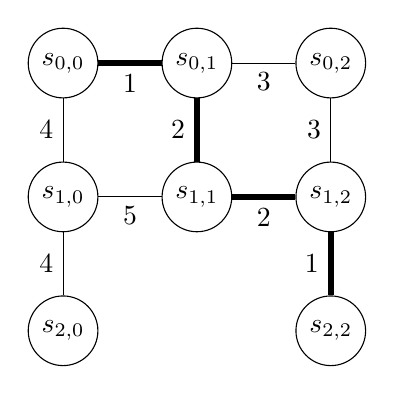
\begin{tikzpicture}
            \tikzset{Vertex/.style={%
                shape=circle,%
                draw=black,%
                minimum size=10pt,%
                radius=1cm,%
                inner sep=3pt,%
                node distance=1.7cm,%
            }}
    
            \node[Vertex] (v00) at (0,0) {$s_{0,0}$};
            \node[Vertex, right of=v00] (v01) {$s_{0,1}$};
            \node[Vertex, right of=v01] (v02) {$s_{0,2}$};
            \node[Vertex, below of=v00] (v10) {$s_{1,0}$};
            \node[Vertex, right of=v10] (v11) {$s_{1,1}$};
            \node[Vertex, right of=v11] (v12) {$s_{1,2}$};
            \node[Vertex, below of=v10] (v20) {$s_{2,0}$};
            \node[Vertex, below of=v12] (v22) {$s_{2,2}$};
    
            \path (v00) edge[-.,line width=2pt] node[below]{1} (v01);
            \path (v01) edge[-.] node[below]{3} (v02);
            \path (v10) edge[-.] node[below]{5} (v11);
            \path (v11) edge[-.,line width=2pt] node[below]{2} (v12);
            \path (v00) edge[-.] node[left]{4} (v10);
            \path (v10) edge[-.] node[left]{4} (v20);
            \path (v01) edge[-.,line width=2pt] node[left]{2} (v11);
            \path (v02) edge[-.] node[left]{3} (v12);
            \path (v12) edge[-.,line width=2pt] node[left]{1} (v22);
        \end{tikzpicture}
        $$s_{0,0} \rightarrow s_{0,1} \rightarrow s_{1,1} \rightarrow s_{1,2} \rightarrow s_{2,2}$$
    \end{minipage}
\end{frame}

\begin{frame}[fragile]{A simple example}
    \begin{center}
        \textbf{Perturbated Map}\\
    \end{center}

    \begin{minipage}{0.5\textwidth}
        \begin{tikzpicture}
            \matrix[square matrix]{
                |[fill=black!0]| $s_{0,0}$   &|[fill=black!0]| $s_{0,1}$  &|[fill=black!40]| $s_{0,2}$  \\
                |[fill=black!60]| $s_{1,0}$   &|[fill=black!60]| $s_{1,1}$  &|[fill=black!0]| $s_{1,2}$  \\
                |[fill=black!0]| $s_{2,0}$   &|[fill=black]|  &|[fill=black!0]| $s_{2,2}$  \\
            };
        \end{tikzpicture}
        
        \begin{tabular}{clcl}
            \drawFilledSquare{black!0} & 1 &
            \drawFilledSquare{black!20} & 3 \\
            \drawFilledSquare{black!40} & 5 &
            \drawFilledSquare{black!60} & 7 \\
            \drawFilledSquare{black} & $\infty$ &
            & \\
        \end{tabular}
    \end{minipage}%
    \begin{minipage}{0.5\textwidth}
        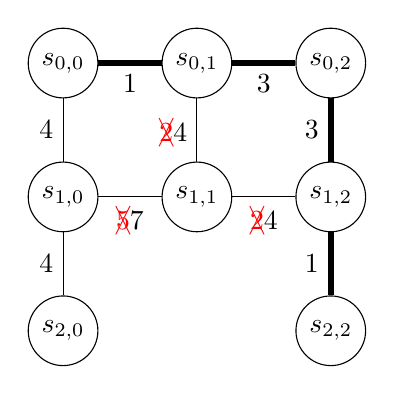
\begin{tikzpicture}
            \tikzset{Vertex/.style={%
                shape=circle,%
                draw=black,%
                minimum size=10pt,%
                radius=1cm,%
                inner sep=3pt,%
                node distance=1.7cm,%
            }}
    
            \node[Vertex] (v00) at (0,0) {$s_{0,0}$};
            \node[Vertex, right of=v00] (v01) {$s_{0,1}$};
            \node[Vertex, right of=v01] (v02) {$s_{0,2}$};
            \node[Vertex, below of=v00] (v10) {$s_{1,0}$};
            \node[Vertex, right of=v10] (v11) {$s_{1,1}$};
            \node[Vertex, right of=v11] (v12) {$s_{1,2}$};
            \node[Vertex, below of=v10] (v20) {$s_{2,0}$};
            \node[Vertex, below of=v12] (v22) {$s_{2,2}$};
    
            \path (v00) edge[-.,line width=2pt] node[below]{1} (v01);
            \path (v01) edge[-.,line width=2pt] node[below]{3} (v02);
            \path (v10) edge[-.] node[below]{{\color{red} \xcancel{5}}{7}} (v11);
            \path (v11) edge[-.] node[below]{{\color{red} \xcancel{2}}{4}} (v12);
            \path (v00) edge[-.] node[left]{4} (v10);
            \path (v10) edge[-.] node[left]{4} (v20);
            \path (v01) edge[-.] node[left]{{\color{red} \xcancel{2}}{4}} (v11);
            \path (v02) edge[-.,line width=2pt] node[left]{3} (v12);
            \path (v12) edge[-.,line width=2pt] node[left]{1} (v22);
        \end{tikzpicture}
        $$s_{0,0} \rightarrow s_{0,1} \rightarrow s_{0,2} \rightarrow s_{1,2} \rightarrow s_{2,2}$$
    \end{minipage}
\end{frame}

\begin{frame}{Talk Outline}
    \begin{itemize}
        \item Context and Background:
        \begin{itemize}
            \item Compress Path Database (\CPD{});
            \item \ALT{}, \AWA{};
        \end{itemize}
        \item Proposed Techniques: \CPDSearch{} and \anytimeCPDSearch{};
        \item Experimental Results: 
            \begin{itemize}
                \item optimal and 
                \item anytime scenario;
            \end{itemize}
        \item Conclusion and Future Work;
    \end{itemize}
\end{frame}
\section*{Background}

\begin{frame}{Context}
    \begin{itemize}
        \item Path planning episodes are independent;
        \item each episode has fixed start and target locations;
        \item graph map is known a priori.
    \end{itemize}
    
    \medskip
    Map edge costs changes (\textit{perturbations}):
    \begin{itemize}
        \item[-] distribution over map unknown a priori;
        \item[-] \textbf{only increase} original edge costs (\eg{} routing in road networks, videogames);
        \item[-] detected at the beginning of each path planning episode and then assumed fixed.
    \end{itemize}
\end{frame}

\begin{frame}{Compressed Path Database (\CPD{}) [Strasser 2014 + others]}
    \vspace{-8pt}
    \begin{block}{}
       Given a graph, a CPD is a data structure that efficiently stores the first edge of an optimal path from any node $s$ towards any node $t$.
    \end{block}

    \vspace{-2pt}
    \begin{minipage}{0.33\textwidth}
        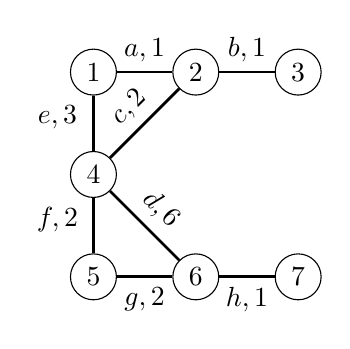
\begin{tikzpicture}
            \tikzset{Vertex/.style={%
                    shape=circle,%
                    draw=black,%
                    minimum size=10pt,%
                    radius=1cm,%
                    inner sep=3pt,%
                    node distance=1.3cm,%
                }}
        
                \node[Vertex] (1) {$1$};
                \node[Vertex, right of=1] (2) {$2$};
                \node[Vertex, right of=2] (3) {$3$};
                \node[Vertex, below of=1] (4) {$4$};
                \node[Vertex, below of=4] (5) {$5$};
                \node[Vertex, right of=5] (6) {$6$};
                \node[Vertex, right of=6] (7) {$7$};
        
                \path (1) edge[-,line width=1pt] node[above]{$a,1$} (2);
                \path (2) edge[-,line width=1pt] node[above]{$b,1$} (3);
                \path (4) edge[-,line width=1pt] node[above,sloped]{$c,2$} (2);
                \path (4) edge[-,line width=1pt] node[above,sloped]{$d,6$} (6);
                \path (4) edge[-,line width=1pt] node[above,xshift=-13pt,yshift=-6pt]{$e,3$} (1);
                \path (4) edge[-,line width=1pt] node[above,xshift=-13pt, yshift=-6pt]{$f,2$} (5);
                \path (5) edge[-,line width=1pt] node[below]{$g,2$} (6);
                \path (6) edge[-,line width=1pt] node[below]{$h,1$} (7);
        \end{tikzpicture}%
        \begin{center}%
            \vspace{-13pt}%
            $(s,t) = (2, 6)$%
        \end{center}
    \end{minipage}\hfill%
    \begin{minipage}{0.50\textwidth}
        \begin{center}
            \begin{minipage}{1.0\textwidth}
                \begin{minipage}{0.5\textwidth}
                    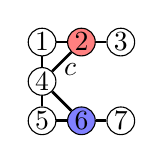
\begin{tikzpicture}
                        \tikzset{Vertex/.style={%
                                shape=circle,%
                                draw=black,%
                                minimum size=10pt,%
                                inner sep=0pt,%
                                node distance=0.5cm,%
                            }}
                    
                            \node[Vertex] (1) {$1$};
                            \node[Vertex, fill=red!50, right of=1] (2) {$2$};
                            \node[Vertex, right of=2] (3) {$3$};
                            \node[Vertex, below of=1] (4) {$4$};
                            \node[Vertex, below of=4] (5) {$5$};
                            \node[Vertex, fill=blue!50, right of=5] (6) {$6$};
                            \node[Vertex, right of=6] (7) {$7$};
                    
                            \path (1) edge[-,line width=1pt] (2);
                            \path (2) edge[-,line width=1pt] (3);
                            \path (4) edge[-,line width=1pt] node[xshift=3pt, yshift=3pt, below]{$c$} (2);
                            \path (4) edge[-,line width=1pt] (6);
                            \path (4) edge[-,line width=1pt] (1);
                            \path (4) edge[-,line width=1pt] (5);
                            \path (5) edge[-,line width=1pt] (6);
                            \path (6) edge[-,line width=1pt] (7);
                    \end{tikzpicture}
                \end{minipage}\hfill%
                \begin{minipage}{0.5\textwidth}
                    $CPD[2,6] = c$
                \end{minipage}

                \begin{minipage}{0.5\textwidth}
                    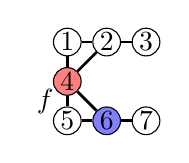
\begin{tikzpicture}
                        \tikzset{Vertex/.style={%
                                shape=circle,%
                                draw=black,%
                                minimum size=10pt,%
                                inner sep=0pt,%
                                node distance=0.5cm,%
                            }}
                    
                            \node[Vertex] (1) {$1$};
                            \node[Vertex, right of=1] (2) {$2$};
                            \node[Vertex, right of=2] (3) {$3$};
                            \node[Vertex, fill=red!50, below of=1] (4) {$4$};
                            \node[Vertex, below of=4] (5) {$5$};
                            \node[Vertex, fill=blue!50, right of=5] (6) {$6$};
                            \node[Vertex, right of=6] (7) {$7$};
                    
                            \path (1) edge[-,line width=1pt] (2);
                            \path (2) edge[-,line width=1pt] (3);
                            \path (4) edge[-,line width=1pt] (2);
                            \path (4) edge[-,line width=1pt] (6);
                            \path (4) edge[-,line width=1pt] (1);
                            \path (4) edge[-,line width=1pt] node[xshift=-8pt]{$f$} (5);
                            \path (5) edge[-,line width=1pt] (6);
                            \path (6) edge[-,line width=1pt] (7);
                    \end{tikzpicture}
                \end{minipage}\hfill%
                \begin{minipage}{0.5\textwidth}
                    $CPD[4,6] = f$
                \end{minipage}

                \begin{minipage}{0.5\textwidth}
                    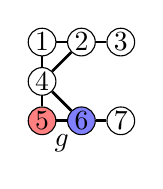
\begin{tikzpicture}
                        \tikzset{Vertex/.style={%
                                shape=circle,%
                                draw=black,%
                                minimum size=10pt,%
                                inner sep=0pt,%
                                node distance=0.5cm,%
                            }}
                    
                            \node[Vertex] (1) {$1$};
                            \node[Vertex, right of=1] (2) {$2$};
                            \node[Vertex, right of=2] (3) {$3$};
                            \node[Vertex, below of=1] (4) {$4$};
                            \node[Vertex, fill=red!50, below of=4] (5) {$5$};
                            \node[Vertex, fill=blue!50, right of=5] (6) {$6$};
                            \node[Vertex, right of=6] (7) {$7$};
                    
                            \path (1) edge[-,line width=1pt] (2);
                            \path (2) edge[-,line width=1pt] (3);
                            \path (4) edge[-,line width=1pt] (2);
                            \path (4) edge[-,line width=1pt] (6);
                            \path (4) edge[-,line width=1pt] (1);
                            \path (4) edge[-,line width=1pt] (5);
                            \path (5) edge[-,line width=1pt] node[yshift=-8pt]{$g$} (6);
                            \path (6) edge[-,line width=1pt] (7);
                    \end{tikzpicture}
                \end{minipage}\hfill%
                \begin{minipage}{0.5\textwidth}
                    $CPD[5,6] = g$
                \end{minipage}
            \end{minipage}

        \end{center}     
    \end{minipage}

    \vspace{-9pt}
    \begin{coloredBlock}{\CPDPathName{}}[OliveGreen][white]
        Given a graph $G$ and its \CPD{}, source node $s$ and target node $t$, 
        the $\CPDPath{s}{t}$ is the path obtained by concatenating edge $\CPD{}[s, t]$ with $\CPDPath{sink(\CPD{}[s, t])}{t}$ if $s \not = t$; the empty path otherwise.
    \end{coloredBlock}

\end{frame}
\section*{Proposed Techniques}

\begin{frame}{Proposed technique: \CPDSearch{}}
    \begin{block}{Idea}
        Exploit the original CPD for the new perturbated map.
    \end{block}

    \begin{itemize}
        \item<2-> {\color<3->{gray}Use CPD as a concrete (suboptimal) solution};
        \item<3-> {\color<4->{gray}use CPD as an admissible heuristic};
        \item<4-> {\color<5->{gray}use CPD for a (early) search termination};
        \item<5-> {use CPD to obtain anytime solution (if weights $\not = \infty$)};
    \end{itemize}

    \only<3>{
        Given start, target $(s, t)$, since perturbations only increases edge costs, the cost of the shortest path computed by the CPD is a lowerbound of the actual shortest path in the perturbated graph;
    }%
    \only<2-3>{
        \begin{minipage}{0.5\textwidth}
            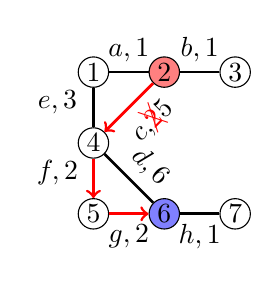
\begin{tikzpicture}
                \tikzset{Vertex/.style={%
                    shape=circle,%
                    draw=black,%
                    minimum size=10pt,%
                    radius=0.7cm,%
                    inner sep=1pt,%
                    node distance=0.9cm,%
                }}
            
                \node[Vertex] (1) {$1$};
                \node[Vertex, right of=1, fill=red!50] (2) {$2$};
                \node[Vertex, right of=2] (3) {$3$};
                \node[Vertex, below of=1] (4) {$4$};
                \node[Vertex, below of=4] (5) {$5$};
                \node[Vertex, right of=5, fill=blue!50] (6) {$6$};
                \node[Vertex, right of=6] (7) {$7$};
        
                \path (2) edge[-,line width=1pt] node[above]{\color{black}$a,1$} (1);
                \path (2) edge[-,line width=1pt] node[above]{\color{black}$b,1$} (3);
                \path (2) edge[->,line width=1pt, color=red] node[below,sloped,pos=0.4]{{\color{black} $c,$}{\color{red} \xcancel{2}}{\color{black}5}} (4);
                \path (4) edge[-,line width=1pt] node[above,sloped,pos=0.6]{\color{black}$d,6$} (6);
                \path (1) edge[-,line width=1pt] node[above,xshift=-13pt,yshift=-6pt]{\color{black}$e,3$} (4);
                \path (4) edge[->,line width=1pt, color=red] node[above,xshift=-13pt, yshift=-6pt]{\color{black}$f,2$} (5);
                \path (5) edge[->,line width=1pt, color=red] node[below]{\color{black}$g,2$} (6);
                \path (6) edge[-,line width=1pt] node[below]{\color{black}$h,1$} (7);
            \end{tikzpicture}
        \end{minipage}\hfill%
        \begin{minipage}{0.5\textwidth}
            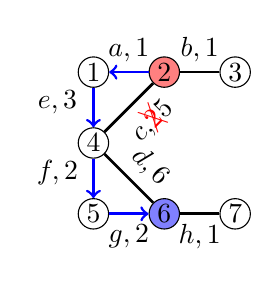
\begin{tikzpicture}
                \tikzset{Vertex/.style={%
                    shape=circle,%
                    draw=black,%
                    minimum size=10pt,%
                    radius=0.7cm,%
                    inner sep=1pt,%
                    node distance=0.9cm,%
                }}
            
                \node[Vertex] (1) {$1$};
                \node[Vertex, right of=1, fill=red!50] (2) {$2$};
                \node[Vertex, right of=2] (3) {$3$};
                \node[Vertex, below of=1] (4) {$4$};
                \node[Vertex, below of=4] (5) {$5$};
                \node[Vertex, right of=5, fill=blue!50] (6) {$6$};
                \node[Vertex, right of=6] (7) {$7$};
        
                \path (2) edge[->,line width=1pt, color=blue] node[above]{\color{black}$a,1$} (1);
                \path (2) edge[-,line width=1pt] node[above]{\color{black}$b,1$} (3);
                \path (2) edge[-,line width=1pt] node[below,sloped,pos=0.4]{{\color{black} $c,$}{\color{red} \xcancel{2}}{\color{black}5}} (4);
                \path (4) edge[-,line width=1pt] node[above,sloped,pos=0.6]{\color{black}$d,6$} (6);
                \path (1) edge[->,line width=1pt, color=blue] node[above,xshift=-13pt,yshift=-6pt]{\color{black}$e,3$} (4);
                \path (4) edge[->,line width=1pt, color=blue] node[above,xshift=-13pt, yshift=-6pt]{\color{black}$f,2$} (5);
                \path (5) edge[->,line width=1pt, color=blue] node[below]{\color{black}$g,2$} (6);
                \path (6) edge[-,line width=1pt] node[below]{\color{black}$h,1$} (7);
            \end{tikzpicture}
        \end{minipage}
    }%
    \only<4>{
        \begin{minipage}{0.5\textwidth}
            \begin{flushleft}
                path in original map: 6 \\
                path in perturbated map: 9
            \end{flushleft}
            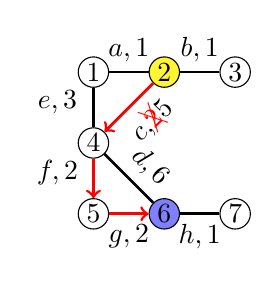
\begin{tikzpicture}
                \tikzset{Vertex/.style={%
                    shape=circle,%
                    draw=black,%
                    minimum size=10pt,%
                    radius=0.7cm,%
                    inner sep=1pt,%
                    node distance=0.9cm,%
                }}
            
                \node[Vertex] (1) {$1$};
                \node[Vertex, right of=1, fill=yellow!80] (2) {$2$};
                \node[Vertex, right of=2] (3) {$3$};
                \node[Vertex, below of=1] (4) {$4$};
                \node[Vertex, below of=4] (5) {$5$};
                \node[Vertex, right of=5, fill=blue!50] (6) {$6$};
                \node[Vertex, right of=6] (7) {$7$};
        
                \path (2) edge[-,line width=1pt] node[above]{\color{black}$a,1$} (1);
                \path (2) edge[-,line width=1pt] node[above]{\color{black}$b,1$} (3);
                \path (2) edge[->,line width=1pt, color=red] node[below,sloped,pos=0.4]{{\color{black} $c,$}{\color{red} \xcancel{2}}{\color{black}5}} (4);
                \path (4) edge[-,line width=1pt] node[above,sloped,pos=0.6]{\color{black}$d,6$} (6);
                \path (1) edge[-,line width=1pt] node[above,xshift=-13pt,yshift=-6pt]{\color{black}$e,3$} (4);
                \path (4) edge[->,line width=1pt, color=red] node[above,xshift=-13pt, yshift=-6pt]{\color{black}$f,2$} (5);
                \path (5) edge[->,line width=1pt, color=red] node[below]{\color{black}$g,2$} (6);
                \path (6) edge[-,line width=1pt] node[below]{\color{black}$h,1$} (7);
            \end{tikzpicture}
        \end{minipage}\hfill%
        \begin{minipage}{0.5\textwidth}
            \begin{flushleft}
                path in original map: 7 \\
                path in perturbated map: 7
            \end{flushleft}
            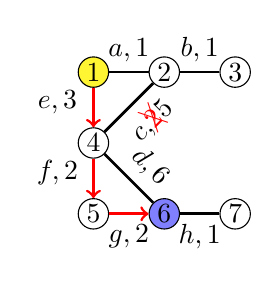
\begin{tikzpicture}
                \tikzset{Vertex/.style={%
                    shape=circle,%
                    draw=black,%
                    minimum size=10pt,%
                    radius=0.7cm,%
                    inner sep=1pt,%
                    node distance=0.9cm,%
                }}
            
                \node[Vertex, fill=yellow!80] (1) {$1$};
                \node[Vertex, right of=1] (2) {$2$};
                \node[Vertex, right of=2] (3) {$3$};
                \node[Vertex, below of=1] (4) {$4$};
                \node[Vertex, below of=4] (5) {$5$};
                \node[Vertex, right of=5, fill=blue!50] (6) {$6$};
                \node[Vertex, right of=6] (7) {$7$};
        
                \path (2) edge[-,line width=1pt] node[above]{\color{black}$a,1$} (1);
                \path (2) edge[-,line width=1pt] node[above]{\color{black}$b,1$} (3);
                \path (2) edge[-,line width=1pt] node[below,sloped,pos=0.4]{{\color{black} $c,$}{\color{red} \xcancel{2}}{\color{black}5}} (4);
                \path (4) edge[-,line width=1pt] node[above,sloped,pos=0.6]{\color{black}$d,6$} (6);
                \path (1) edge[->,line width=1pt, color=red] node[above,xshift=-13pt,yshift=-6pt]{\color{black}$e,3$} (4);
                \path (4) edge[->,line width=1pt, color=red] node[above,xshift=-13pt, yshift=-6pt]{\color{black}$f,2$} (5);
                \path (5) edge[->,line width=1pt, color=red] node[below]{\color{black}$g,2$} (6);
                \path (6) edge[-,line width=1pt] node[below]{\color{black}$h,1$} (7);
            \end{tikzpicture}
        \end{minipage}
    }%
    \only<5>{
        \begin{minipage}{0.65\textwidth}
            For every search node $n$, CPD allows us to track an incumbent solution which is the shortest such path we have found (\textit{upperbound}).
        \end{minipage}\hfill%
        \begin{minipage}{0.35\textwidth}
            \begin{center}
                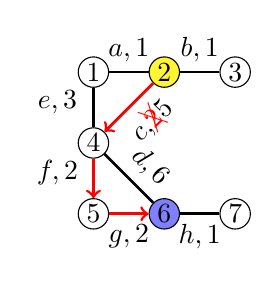
\begin{tikzpicture}
                    \tikzset{Vertex/.style={%
                        shape=circle,%
                        draw=black,%
                        minimum size=10pt,%
                        radius=0.7cm,%
                        inner sep=1pt,%
                        node distance=0.9cm,%
                    }}
                
                    \node[Vertex] (1) {$1$};
                    \node[Vertex, right of=1, fill=yellow!80] (2) {$2$};
                    \node[Vertex, right of=2] (3) {$3$};
                    \node[Vertex, below of=1] (4) {$4$};
                    \node[Vertex, below of=4] (5) {$5$};
                    \node[Vertex, right of=5, fill=blue!50] (6) {$6$};
                    \node[Vertex, right of=6] (7) {$7$};
            
                    \path (2) edge[-,line width=1pt] node[above]{\color{black}$a,1$} (1);
                    \path (2) edge[-,line width=1pt] node[above]{\color{black}$b,1$} (3);
                    \path (2) edge[->,line width=1pt, color=red] node[below,sloped,pos=0.4]{{\color{black} $c,$}{\color{red} \xcancel{2}}{\color{black}5}} (4);
                    \path (4) edge[-,line width=1pt] node[above,sloped,pos=0.6]{\color{black}$d,6$} (6);
                    \path (1) edge[-,line width=1pt] node[above,xshift=-13pt,yshift=-6pt]{\color{black}$e,3$} (4);
                    \path (4) edge[->,line width=1pt, color=red] node[above,xshift=-13pt, yshift=-6pt]{\color{black}$f,2$} (5);
                    \path (5) edge[->,line width=1pt, color=red] node[below]{\color{black}$g,2$} (6);
                    \path (6) edge[-,line width=1pt] node[below]{\color{black}$h,1$} (7);
                \end{tikzpicture}
            \end{center}
        \end{minipage}
    }

\end{frame}


\begin{frame}{Proposed technique: \CPDSearch{}}
    \textbf{\CPDSearch{}}. A* variant yielding bounded suboptimal path:
    \begin{itemize}
        \item mantain the search node $I$ with the least cost $u = g[I] + h'$, where $h'$ is the cost of path over new map computed by \CPD{} going from $I$ to $t$;
        \item if $\epsilon f[n] \geq u$, output solution. Path from $n$ to $t$ is computed from querying \CPD{};
        \item if $\epsilon = 1$, \CPDSearch{} is optimal;
    \end{itemize}
    
\end{frame}

\begin{frame}{\CPDSearch{} as anytime algorithm}
    \begin{itemize}
        \item yield incumbents \CPDSearch{} finds;
        \item if all new weights $\not = \infty$ or user do not have hard time constraints, \CPDSearch{} immediately has a solution;
    \end{itemize}
\end{frame}
\section*{Experiments}

\begin{frame}{Experimental Setup}
    
    \begin{itemize}
        \item Benchmark from moving AI [Sturtevant, 2012];
        \item policies used to generate perturbations;
            \begin{itemize}
                \item \code{RANDOM}: randomly choose 10\% of edges whose cost is multiplied by 3;
                \item \code{AREA}: for each query, randomly choose location on optimal path and alter edge-costs in an area with 15 radius by multiplying cost with a decaying function ranging from 4 to 1;
            \end{itemize}
        \item optimal and anytime scenario.
    \end{itemize}
    Comparing techniques:
    \begin{itemize}
        \item[-] \ALT{}: Search technique using preprocessed \textit{landmarks} to derive admissible heuristic for any node pair $(s, t)$ [Goldberg and Harrelson, 2005];
        \item[-] \AWA{}: \WA{} anytime variant iteratively computing suboptimal solutions while updating in the tightest possible way the suboptimality bound [Hansen and Zhou, 2007];
    \end{itemize}
\end{frame}

\begin{frame}{Optimal Scenario}
    \begin{adjustwidth}{-2.5em}{-2.5em}
        \begin{minipage}{0.59\textwidth}
            \begin{figure}
                \centering
                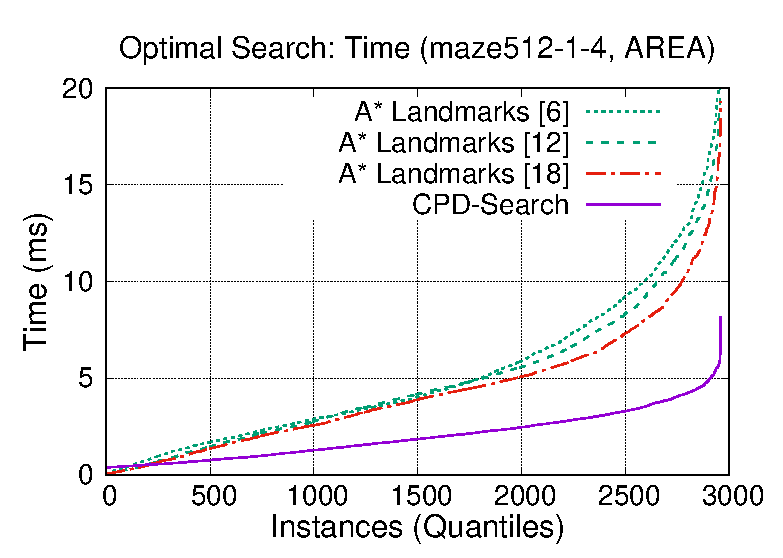
\includegraphics[width=1.0\textwidth]{src/images/optimal/maze512-1-4}
                \label{fig:optimal-maze512-1-4}
            \end{figure}
        \end{minipage}%
        \begin{minipage}{0.59\textwidth}
            \begin{figure}
                \centering
                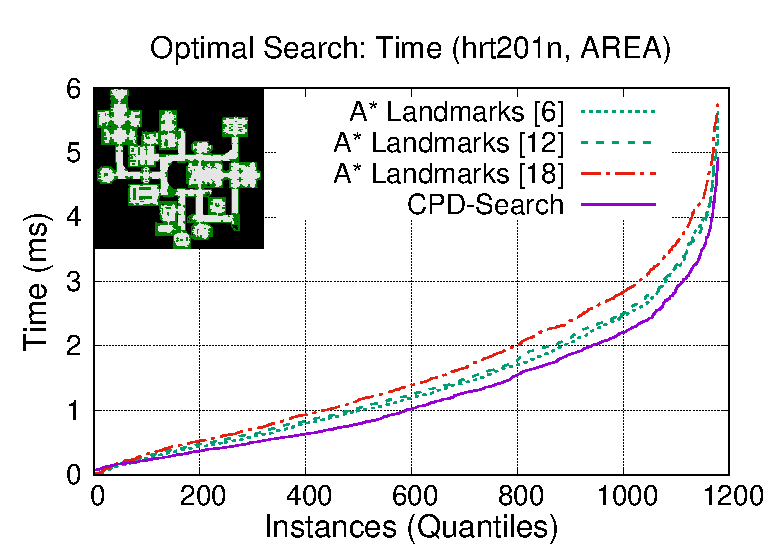
\includegraphics[width=1.0\textwidth]{src/images/optimal/hrt201n}
                \label{fig:optimal-hrt201n}
            \end{figure}
        \end{minipage}
    \end{adjustwidth}
\end{frame}

\begin{frame}{Anytime Scenario}

    In \code{hrt201n} map (almost 1200 queries):

    \begin{itemize}
        \item by 30$\mu$s \anytimeCPDSearch{} has solutions for at least 25\% of instances, \AWA{} for almost 0\%;
        \item by 300$\mu$s \anytimeCPDSearch{} has solutions for at least 75\% of instances, \AWA{} for at most 50\%;
        \item by 1ms \anytimeCPDSearch{} has solutions for all instances and has computed the optimal path for at least 25\% of instances, \AWA{} has optimal paths for no instance;
        \item by 10ms \anytimeCPDSearch{} has reached the optimal solution for every instance, while \AWA{} has computed it for at most 50\%.
    \end{itemize}
\end{frame}

\section*{Conclusions}

\begin{frame}{Conclusions and Future Works}
    \begin{itemize}
        \item Proposed \CPD{}s as heuristic functions for dynamic settings where costs can only increase;
        \item described a new algorithm, \CPDSearch{} which can be used in both optimal and anytime context;
        \item experimentally-evaluated \CPDSearch{} performances shows gain in both contexts over previous state-of-the-art algorithms (\ALT{} and \AWA{});
        \item \textbf{Future Work}: explore \CPD{} usage in Multi-Agent Path Finding context and in dynamically changing edge costs over time.
    \end{itemize}
\end{frame}

\begin{frame}[plain,c]

\begin{center}
    \setFontSize{35}{Thank you for your attention}
\end{center}



\begin{center}
    \setFontSize{35}{Questions?}
\end{center}

\end{frame}


\end{document}
